\documentclass[a4paper]{article}

\usepackage[top=2cm, bottom=2cm, left=3cm, right=3cm]{geometry}
\usepackage[utf8]{inputenc}
\usepackage[english]{babel}
\usepackage{csquotes}
\usepackage[T1]{fontenc}
\usepackage{lmodern}
\usepackage[hidelinks]{hyperref}
\usepackage{graphicx}
\usepackage{url}
\usepackage[indent]{parskip}
\usepackage{microtype}

\title{%
    Fog Project Documentation\\[5mm]
    {\normalsize Edge-Cloud application simulating household power
    consumption\\[-2mm] with robust disconnection handling}
}
\author{Marvin Steinke \and Niklas Fomin}
\date{\today}

\begin{document}
\maketitle

\begin{figure}
    \centering
    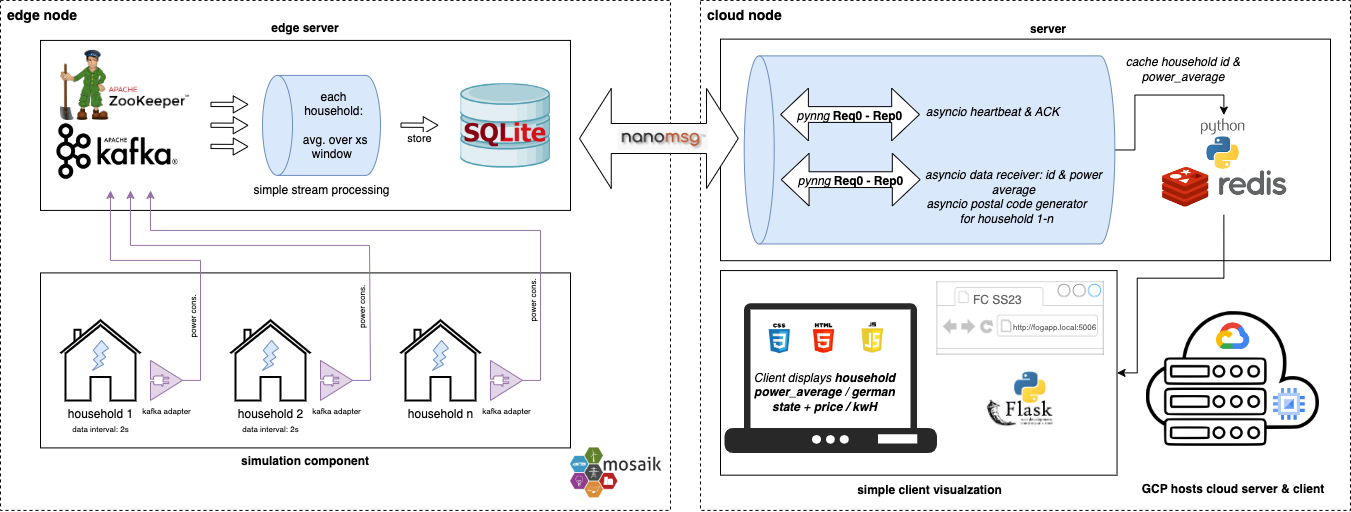
\includegraphics[width=\linewidth]{../schema/schema}
    \caption{Project Schema}
    \label{fig:project_schema}
\end{figure}

This project simulates a distributed power system where power data from
different households is streamed in real-time. The data is processed and
averaged over a 5-second window. The simulation is coordinated by Mosaik, a
co-simulation framework, and uses Apache Kafka for handling real-time data. The
averaged data gets queued into a SQLite database and arranged into a schema
that allows for the tracking of each inserted tuple. The edge server manages the
messaging of the queued data by continuously checking connectivity to the cloud
server and buffering the generated tuples into the sockets. The cloud server
caches each received tuple and generates the corresponding postal code for the
household, and sends this back to the edge server. The edge server eventually
stores this in its database and marks the tuple as acknowledged. The initial
start of the cloud server triggers a backend running on the same hosts that
fetches key-value pairs out of the cache and visualizes them on charts,
accessible on the web. A schema for the project is depicted in Figure
\ref{fig:project_schema}.

\section{Edge Component}

\begin{itemize}

    \item \texttt{data}: Based on the original data from \enquote{Gem House
        Opendata: German Electricity Consumption in Many Households Over Three
    Years 2018-2020 (Fresh Energy)} \cite{milojkovic2021}. The data is reduced
    to a one hour window and made compatible with the simulation environment by
    adding a title and converting the timestamp from \texttt{YYYY-MM-DD
    HH:mm:ss.SSS} to \texttt{YYYY-MM-DD HH:mm:ss}.

    \item \texttt{household.py}: Contains the Household simulator that generates
        power data based on the provided CSV file.

    \item \texttt{kafka\_adapter.py}: Contains the KafkaAdapter and
        KafkaAdapterModel classes, responsible for connecting the Mosaik
        simulation with the Kafka data stream.

    \item \texttt{collector.py}: Contains the Collector simulator that collects
        all power data.

    \item \texttt{main.py}: Contains the main function for starting the
        simulation.

    \item \texttt{edge\_server.py}: Contains the EdgeServer class for reading,
        writing, and inserting the produced data from the Kafka topics into
        SQLite. Additionally, three concurrent threads are used to continuously
        check connectivity, publish data read from the Kafka topics and the
        SQLite database, and subscribe to messages from the cloud server. For
        messaging, we use Pynng, which is a Python wrapper of the lightweight,
        high-performance messaging library nano message. Initially, it does not provide
        \enquote{reliable} features such as message buffering or connection
        retries. It is considered to be based on ZeroMQ but aims to simplify its
        usage. With concerns to reliability the edge server uses the database to
        track if a message was sent or not. Initially the flag is set to 0. If sent it turn 1.
        Only if the server received it and replied with the according postal code of the received ID
        the message is considered acknowledged and the flag is set to 2 and eventually the postal code
        is inserted into the db. Whenever the connection to the cloud node is established the data_sender
        thread wakes up and both fetches both new data with sent flag 0 or data that might be lost with the
        flag 1. This mechanism contributes to the robust disconnection handling. whenever the cloud-node 
        crashes or the connection is dirupted the edge-server will buffer the queued messages to be sent.
        When the edge-server crashes the cloud node logs accordingly and continues retrying to acknowledge 
        heartbeats from the edge side. As soon as the edge-server is back online it benefits of the persistent
        data-storage and continues sending data beginning from the last sent message ID. Again, in case the 
        cloud-node sent the acknowledgement, but the edge-node crashed, as soon as it starts up again it will 
        check the database and resent the unsent or unacknowledged messages to the cloud-node.

    \item \texttt{db\_operations.py}: The database contains operations for the
        lightweight, file-based SQLite database used by the \texttt{EdgeServer}.
        It creates a schema, inserts tuples received from the Kafka producer
        thread, and fetches newly inserted and lost data by tracking and
        checking the \texttt{sent} flag. Furthermore, it handles the insertion
        of messages received from the cloud server.


\end{itemize}

\section{Cloud Node}

The cloud node runs the \texttt{cloud\_server.py} file to interact
asynchronously with the edge component through three pynng sockets, utilizing
both Pub/Sub and Req/Rep message patterns. The cloud node subscribes to the data
from the Kafka server and caches the received data into a Redis cache. It also
publishes the generated postal codes to the edge server and triggers the
\texttt{data\_fetcher.py} script in the backend to fetch data from the cache.
This process provides a RESTful API for an AJAX engine running \texttt{main.js}
in the frontend. The cloud server responds to continuous heartbeat messages to
ensure necessary reliability and handle disconnections in the event of network
failures or application crashes. The cloud server responds to continuous heartbeat
messages to ensure necessary reliability and handle disconnections in the event of 
network failures or application crashes. Both the cloud server and the web client can be operated by 
the startup_script.sh integrated in the terraform files.

\begin{itemize}

    \item \texttt{cloud\_server.py}: Contains asynchronous (implemented with
        asyncio \& pynng) functions that reply to heartbeat messages by the edge-server, receive
        the power data and reply with the generated postal codes back to the
        edge-server. The received data gets cached to redis-server instance on the
        same host.

    \item \texttt{data\_fetcher.py}: Contains the flask backend script to fetch
        data out of the redis-cache, associate one of sixteen german states with
        the id of the received data tuple and providing a REST API for the
        frontend to present the data values on a webpage.

    \item \texttt{main.js + index.html + main.css}: Contains a simple frontend
        logic to access the key-value-pairs using ajax and implements a
        bar-chart of the \texttt{Chart.js} library to visualize the average
        power-consumption per german state in annual kw/h + the associated price
        based on an assumption.

\end{itemize}

\bibliographystyle{IEEEtran}
\bibliography{refs}

\end{document}
